\setcounter{page}{45}
\begin{center}
    {\Large \textbf{Задачи и Вопросы}}
\end{center}

\textbf{3.} Внутри окружности радиуса \( R \) находятся две другие окружности, касающиеся друг друга и данной окружности. Найти периметр треугольника, вершины которого служат центры трёх окружностей.

\vspace{0.5em}

\textbf{4.} Может ли для углов треугольника удовлетворяться равенство:  
\[
\sin A + \sin B = \sin C?
\]

\vspace{0.5em}

\textbf{5.} Возможно ли равенство \( \sin A = \lg \sin \alpha \)?

\vspace{0.5em}

\textbf{6.} Докажите, что треугольник является равнобедренным, если у него равны две медианы.

\vspace{0.5em}

\textbf{7.} Докажите, что для произвольной трапеции \( ABCD \) справедливо равенство:  
\[
AO \cdot BO = DO \cdot CO,
\]
где \( O \) — точка пересечения диагоналей \( AC \) и \( BD \).

\vspace{0.5em}

\textbf{8.} Полуокружность радиуса \( R \) разделена на три равные части, и точки деления соединены с одним из концов диаметра, стягивающего эту полуокружность. Найти площадь, ограниченную двумя хордами и заключённую между ними дугой.

\vspace{0.5em}

\textbf{9.} В некоторой пирамиде двугранные углы при основании равны $\alpha$, и площадь основания $S$. Найти площадь боковой поверхности.

\section*{Вопросы второго уровня}

\textbf{1*.} Найти множество точек плоскости \( M(x, y) \), координаты которых удовлетворяют уравнению:  
\[
\sin x + \sin y = \frac{x}{\left|x\right|} + \frac{y}{\left|y\right|}.
\]

\vspace{0.5em}

\textbf{2*.} Решить уравнение:  
\[
\tg x + \ctg x = -1.75.
\]

\vspace{0.5em}

\textbf{3*.} Решить неравенство:  
\[
2^{3x} + 3^{2x} - 2\cdot11x > 0.
\]

\vspace{0.5em}

\textbf{4*.} При каких условиях квадратный трёхчлен \( ax^2 + bx + c \) (\( a \neq 0 \)) с действительными коэффициентами является квадратом линейного двучлена с действительными коэффициентами?

\vspace{0.5em}

\textbf{5*.} Сколько сфер можно провести через три точки в пространстве?

\vspace{0.5em}

\textbf{6*.} Можно ли пересечь плоскостью параллелепипед таким образом, чтобы в сечении получился правильный пятиугольник?


\section* \small{Указание. Применить теорему о пересечении двух параллельных плоскостей третьей плоскостью}

\vspace{0.5em}

\textbf{7*.} Треугольник \( ABC \) — остроугольный, \( \angle A = \alpha \). На стороне \( BC \), как на диаметре, описана полуокружность. \( P \) и \( Q \) — точки пересечения этой полуокружности со сторонами \( AB \) и \( AC \) соответственно. Найти отношение площадей треугольников \( ABC \) и \( PAQ \).

\vspace{0.5em}

\textbf{8*.} На сторонах произвольного выпуклого четырёхугольника как на диаметре построены круги. Доказать, что они покрывают весь четырёхугольник.

\vspace{0.5em}

\textbf{9*.} Найти первые три десятичных знака числа \( 7 \cdot 0.999 \).

\vspace{0.5em}

\textbf{10*.}  
а) Существует ли восьмиугольная пирамида, у которой все рёбра равны?  
б) Для каких \( n \) существует правильная \( n \)-угольная пирамида, у которой все рёбра равны?

\vspace{0.5em}

\textbf{11*.} В параллелограмме \( ABCD \) точки \( M \) и \( N \) — середины сторон \( BC \) и \( CD \) соответственно. Доказать, что отрезки \( AM \) и \( AN \) делят диагональ \( BD \) на три равные части.

\vspace{0.5em}

\textbf{12*.} В угол вписаны две окружности: \(A \) и \(B \) - одна касается сторон угла, а другая — вписанная в треугольник с вершиной в углу. Доказать, что отрезок, соединяющий центры окружностей, проходит через точку касания.

\vspace{0.5em}

\textbf{13*.} Построить треугольник, если даны: прямая, на которой лежит основание, и две точки — основания высот, опущенных на боковые стороны.

\vspace{0.5em}

\textbf{14*.} Существует ли треугольник, у которого:  

а) биссектрисы лежат на одной прямой;  
б) высоты лежат на одной прямой?


\small Указание. Продумайте различие между пунктами а) и б)

\vspace{0.5em}

\textbf{15*.} Доказать, что $tg 5°$ - иррациональное число.

\begin{figure}[H]
\centering
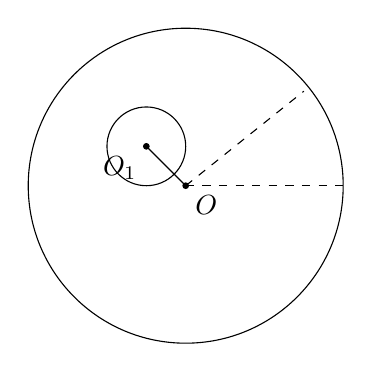
\begin{tikzpicture}

\draw (0,0) circle (2cm);

\draw (-0.5,0.5) circle (0.5cm);

\draw[dashed] (0,0) -- (2,0); 
\draw[dashed] (0,0) -- (1.5,1.2); 

\filldraw (0,0) circle (1pt) node[below right] {$O$}; 
\filldraw (-0.5,0.5) circle (1pt) node[below left] {$O_1$}; 
\draw (-0.5,0.5) -- (0,0);

\end{tikzpicture}
\caption{Рис. 1.}
\end{figure}

\begin{figure}[H]
\centering
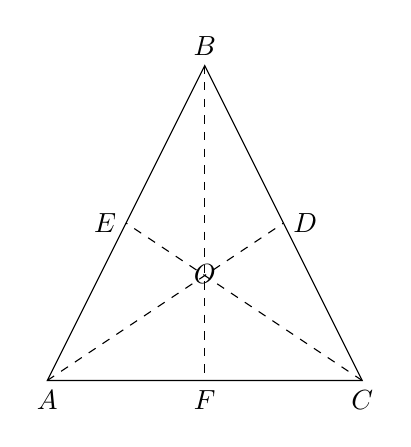
\begin{tikzpicture}
% 定义三角形的顶点
\coordinate (A) at (0,0);
\coordinate (B) at (2,4);
\coordinate (C) at (4,0);
\coordinate (O) at (2,1.6);
\coordinate (E) at (1,2);
\coordinate (D) at (3,2);
\coordinate (F) at (2,0);

% 三角形
\draw (A) -- (B) -- (C) -- cycle;

% 中线
\draw[dashed] (B) -- (F); % BF
\draw[dashed] (C) -- (E); % CE
\draw[dashed] (A) -- (D); % AD

% 点的标记
\draw (A) node[below] {$A$};
\draw (B) node[above] {$B$};
\draw (C) node[below] {$C$};
\draw (F) node[below] {$F$};
\draw (D) node[right] {$D$};
\draw (E) node[left] {$E$};
\draw (O) node[below] {$O$};
\end{tikzpicture}
\caption{Рис. 2.}
\end{figure}

\begin{figure}[H]
\centering
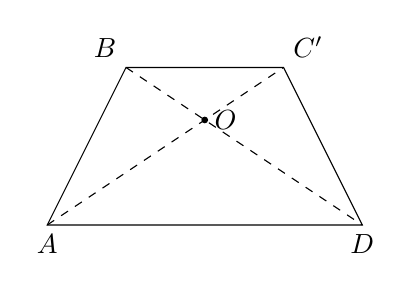
\begin{tikzpicture}
% 定义梯形的顶点
\coordinate (A) at (0,0);
\coordinate (B) at (1,2);
\coordinate (C) at (3,2);
\coordinate (D) at (4,0);
\coordinate (O) at (2,4/3);

% 梯形
\draw (A) -- (B) -- (C) -- (D) -- cycle;

% 对角线
\draw[dashed] (A) -- (C);
\draw[dashed] (B) -- (D);

% 圆心 O
\filldraw (O) circle (1pt) node[right] {$O$};

% 标记点
\draw (A) node[below] {$A$};
\draw (B) node[above left] {$B$};
\draw (C) node[above right] {$C'$};
\draw (D) node[below] {$D$};
\end{tikzpicture}
\caption{Рис. 3.}
\end{figure}